\medskip

Puisqu'on choisit un jouet au hasard dans la production, on est en situation d'équiprobabilité, et donc les proportions sont assimilables à des probabilités.

\medskip

\textbf{Partie A}

\begin{enumerate}
	\item D'après l'énoncé $95\,\%$ des jouets réussissent le test de fabrication et, parmi les jouets qui réussissent le test de fabrication, $98\,\%$ réussissent le test de sécurité, donc  $P(F) = 0,95$ et $P_{F}(S) = 0,98$.

	\item
	\begin{enumerate}
		\item Un arbre pondéré qui illustre la situation avec les données disponibles dans l'énoncé (ainsi que les probabilités d'évènement contraire, triviales) est :

	\hfill~
	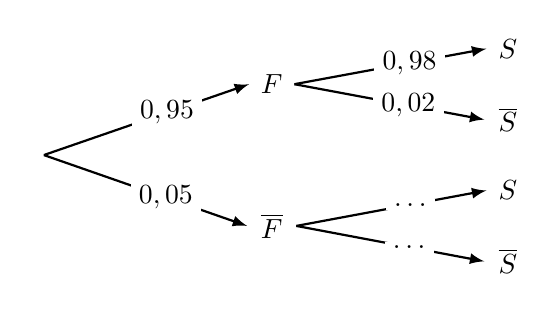
\begin{tikzpicture}[xscale=1,yscale=1,baseline={(R.base)}]
		\tikzstyle{fleche}=[->,>=latex,thick]
		\tikzstyle{noeud}=[fill=white,circle,inner sep=2pt]
		\tikzstyle{feuille}=[fill=white,circle,inner sep=2pt]
		\tikzstyle{etiquette}=[pos=0.6,fill=white, inner xsep=3pt, inner ysep=1.5pt]
		\def\DistanceInterNiveaux{3}
		\def\DistanceInterFeuilles{0.9}
		\def\NiveauA{(0)*\DistanceInterNiveaux}
		\def\NiveauB{(1)*\DistanceInterNiveaux}
		\def\NiveauC{(2)*\DistanceInterNiveaux}
		\def\InterFeuilles{(-1)*\DistanceInterFeuilles}
		
		\node[noeud] (R) at ({\NiveauA},{(1.5)*\InterFeuilles}) {};
		\node[noeud] (Ra) at ({\NiveauB},{(0.5)*\InterFeuilles}) {$F$};
		\node[feuille] (Raa) at ({\NiveauC},{(0)*\InterFeuilles}) {$S$};
		\node[feuille] (Rab) at ({\NiveauC},{(1)*\InterFeuilles}) {$\overline{S}$};
		\node[noeud] (Rb) at ({\NiveauB},{(2.5)*\InterFeuilles}) {$\overline{F}$};
		\node[feuille] (Rba) at ({\NiveauC},{(2)*\InterFeuilles}) {$S$};
		\node[feuille] (Rbb) at ({\NiveauC},{(3)*\InterFeuilles}) {$\overline{S}$};
		
		\draw[fleche] (R.east)--(Ra.west) node[etiquette] {$0,95$};
		\draw[fleche] (Ra.east)--(Raa.west) node[etiquette] {$0,98$};
		\draw[fleche] (Ra.east)--(Rab.west) node[etiquette] {$0,02$};
		\draw[fleche] (R.east)--(Rb.west) node[etiquette] {$0,05$};
		\draw[fleche] (Rb.east)--(Rba.west) node[etiquette] {$\ldots$};
		\draw[fleche] (Rb.east)--(Rbb.west) node[etiquette] {$\ldots$};
	\end{tikzpicture} \hfill~

		\item D'après l'énoncé $1\,\%$ des jouets ne réussissent aucun des deux tests donc $P\big(\,\overline{F}\cap \overline{S}\big)= 0,01$.

$P_{\overline{F}}\big(\overline{S}\big)= \dfrac{P\big(\,\overline{F}\cap \overline{S}\big)}{P\big(\,\overline{F}\big)}  = \dfrac{0,01}{0,05}=0,2$

L'arbre complet est donc :

		\hfill~
		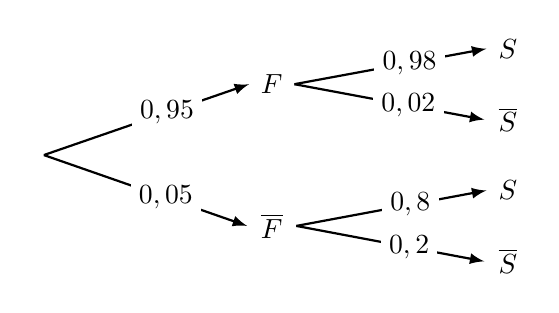
\begin{tikzpicture}[xscale=1,yscale=1,baseline={(R.base)}]
			
			\tikzstyle{fleche}=[->,>=latex,thick]
			\tikzstyle{noeud}=[fill=white,circle,inner sep=2pt]
			\tikzstyle{feuille}=[fill=white,circle,inner sep=2pt]
			\tikzstyle{etiquette}=[pos=0.6,fill=white, inner xsep=3pt, inner ysep=1.5pt]
			
			\def\DistanceInterNiveaux{3}
			\def\DistanceInterFeuilles{0.9}
			
			\def\NiveauA{(0)*\DistanceInterNiveaux}
			\def\NiveauB{(1)*\DistanceInterNiveaux}
			\def\NiveauC{(2)*\DistanceInterNiveaux}
			\def\InterFeuilles{(-1)*\DistanceInterFeuilles}
			
			\node[noeud] (R) at ({\NiveauA},{(1.5)*\InterFeuilles}) {};
			\node[noeud] (Ra) at ({\NiveauB},{(0.5)*\InterFeuilles}) {$F$};
			\node[feuille] (Raa) at ({\NiveauC},{(0)*\InterFeuilles}) {$S$};
			\node[feuille] (Rab) at ({\NiveauC},{(1)*\InterFeuilles}) {$\overline{S}$};
			\node[noeud] (Rb) at ({\NiveauB},{(2.5)*\InterFeuilles}) {$\overline{F}$};
			\node[feuille] (Rba) at ({\NiveauC},{(2)*\InterFeuilles}) {$S$};
			\node[feuille] (Rbb) at ({\NiveauC},{(3)*\InterFeuilles}) {$\overline{S}$};
			
			\draw[fleche] (R.east)--(Ra.west) node[etiquette] {$0,95$};
			\draw[fleche] (Ra.east)--(Raa.west) node[etiquette] {$0,98$};
			\draw[fleche] (Ra.east)--(Rab.west) node[etiquette] {$0,02$};
			\draw[fleche] (R.east)--(Rb.west) node[etiquette] {$0,05$};
			\draw[fleche] (Rb.east)--(Rba.west) node[etiquette] {$0,8$};
			\draw[fleche] (Rb.east)--(Rbb.west) node[etiquette] {$0,2$};
		\end{tikzpicture}~\hfill~
	\end{enumerate}

	\item $P\big(\,F\cap S)  = P(F) \times  P_{F}(S)=0,95 \times 0,98 = 0,931$

	La probabilité que le jouet choisi réussisse les deux tests est égale à $0,931$.

	\item Les évènements $F$ et $\overline{F}$ forment une partition de l'univers, donc, d'après la formule des probabilités totales : \quad $P(S) = P\big(\,F\cap S\big) + P\big(\,\overline{F}\cap S\big) $

On a donc : \quad $P(S)=0,931 + 0,05\times 0,8 = 0,971$.

La probabilité que le jouet réussisse le test de sécurité vaut, $0,97$ arrondi au centième.

	\item $P_{S}(F)= \dfrac{P(F\cap S)}{P(S)} = \dfrac{0,931}{0,971}\approx \np{0,9588}$

La probabilité qu'un jouet  réussisse le test de fabrication  sachant qu'il a réussi le test de sécurité vaut $0,96$, arrondi au centième.
\end{enumerate}

\medskip

\textbf{Partie B}

\medskip

\begin{enumerate}
	\item $S_{n}$ suit la loi binomiale de paramètres $n$ et $p = 0,95$ donc :

$E\left(S_n\right)=n\times p = 0,95n$ \quad et \quad $V(X)=np(1-p)= n \times 0,95 \times 0,05 = \np{0,0475}n$.

	\item Dans cette question, on pose $n = 150$.
	\begin{enumerate}
		\item
		$\begin{aligned}[t] P\left(S_{150}=145\right)
			& = \displaystyle \binom{150}{145}\times 0,95^{145}\times 0,05^{150 - 145}\\
			& = \np{591600030}\times 0,95^{145} \times 0,05^{5}\\
			& \approx \np{0,10884}
		\end{aligned}$.

Finalement, avec les consignes d'arrondi : \quad $P\left(S_{150}= 145\right) \approx 0,109$

Dans le contexte de l'exercice, dans environ 10,9\% des cas, 145 jouets sur les 150 du lot réussissent le test de fabrication.
		\item $94\%$ des jouets de ce lot  correspond à 141 jouets.

À l'aide de la calculatrice : $P\left(S_{150} \geqslant 141\right) \approx \np{0,78088}$

		La probabilité qu'au moins $94\%$ des jouets de ce lot réussissent le test de fabrication vaut $0,781$ à $10^{-3}$ près.
	\end{enumerate}

	\item Dans cette question, l'entier naturel non nul $n$ n'est plus fixé.

	\begin{enumerate}
		\item D'après les propriétés sur l'espérance d'une somme de variables aléatoires :

$E\big(\,F_{n}\big)= E\left(\dfrac{S_{n}}{n}\right) = \dfrac{E\left( S_{n}\right)}{n}= \dfrac{0,95n}{n}= 0,95 $.

D'après les propriétés sur la variance d'une somme de variables aléatoires indépendantes :

$V\big(\,F_{n}\big)= V\left(\dfrac{S_{n}}{n}\right) = \dfrac{V\left( S_{n}\right)}{n^2}= \dfrac{\np{0,0475}n}{n^2}= \dfrac{0,0475}{n}$.

	\item L'évènement \og $0,93 <F_{n}< 0,97$ \fg{} revient à $\big|F_{n} - 0,95 \big| < 0,02$ et

$P\Big(\big|F_n - 0,95 \big| < 0,02\Big) = 1 - P\Big(\big|F_{n} - 0,95 \big| \geqslant 0,02\Big)$.

On veut que $P\Big(\big|F_{n} - 0,95 \big| \geqslant 0,02\Big) \geqslant 0,96$

On veut donc que $P\Big(\big|F_n - 0,95 \big| < 0,02\Big) \leqslant 0,04$

Or, pour tout réel $t > 0$, d'après l'inégalité de Bienaymé-Tchebychev, on a :

$P\Big(\big|F_n-E\big(\,F_n\big)\big| \geqslant t\Big) \leqslant \dfrac{V\big(\,F_n\big)}{t^2}$

Pour $t = 0,02$ on obtient : $ P\Big(\big|F_n-0,95\big| \geqslant 0,02\Big)\leqslant \dfrac{0,475}{ n \times 0,02^2}$.

On veut donc que :\quad $\begin{aligned}[t]
		\dfrac{475}{4 n} \leqslant 0,04 &\iff
		\dfrac{11875}{4} \leqslant n \\
		&\iff 2968+\dfrac{3}{4}\leqslant n
	\end{aligned}$

L'inégalité est donc vraie pour tout entier $n \geqslant \np{2969}$.

À partir de $\np{2969}$ jouets prélevés, la probabilité de l'évènement $I$ est supérieure ou égale à $0,96$.
	\end{enumerate}
\end{enumerate}

\medskip
